\documentclass[review]{elsarticle}

\usepackage{lineno,hyperref}
\usepackage{algorithm}
\usepackage{algorithmic}
\usepackage{amsmath,amssymb}
\usepackage{graphicx}
\usepackage{subfig}
\usepackage{tabularx}
\usepackage[usenames,dvipsnames]{xcolor}
\usepackage{colortbl}
\modulolinenumbers[5]

\journal{CIRP Journal of Manufacturing Science and Technology}

%%%%%%%%%%%%%%%%%%%%%%%
%% Elsevier bibliography styles
%%%%%%%%%%%%%%%%%%%%%%%
%% To change the style, put a % in front of the second line of the current style and
%% remove the % from the second line of the style you would like to use.
%%%%%%%%%%%%%%%%%%%%%%%

%% Numbered
%\bibliographystyle{model1-num-names}

%% Numbered without titles
%\bibliographystyle{model1a-num-names}

%% Harvard
%\bibliographystyle{model2-names.bst}\biboptions{authoryear}

%% Vancouver numbered
%\usepackage{numcompress}\bibliographystyle{model3-num-names}

%% Vancouver name/year
%\usepackage{numcompress}\bibliographystyle{model4-names}\biboptions{authoryear}

%% APA style
%\bibliographystyle{model5-names}\biboptions{authoryear}

%% AMA style
%\usepackage{numcompress}\bibliographystyle{model6-num-names}

%% `Elsevier LaTeX' style
\bibliographystyle{elsarticle-num}
%%%%%%%%%%%%%%%%%%%%%%%

\begin{document}

\begin{frontmatter}

\title{A Spatial AR System for Axis-aligned Augmentation of Planar Scenes in Industrial Settings} %\title{Elsevier \LaTeX\ template\tnoteref{mytitlenote}}
%\tnotetext[mytitlenote]{Fully documented templates are available in the elsarticle package on \href{http://www.ctan.org/tex-archive/macros/latex/contrib/elsarticle}{CTAN}.}

%% Group authors per affiliation:
\author{Michael Horn\'{a}\v{c}ek}\corref{mycorrespondingauthor}
\cortext[mycorrespondingauthor]{Corresponding author}
\ead{michael.hornacek@tuwien.ac.at}
\author{Hans K\"{u}ffner-McCauley}
\author{Majesa Trimmel}
\author{Patrick Rupprecht}
\author{Sebastian Schlund}
\address{Human Centered Cyber Physical Production and Assembly Systems, Institute for Management Sciences, TU Vienna, Austria}

\begin{abstract}
Augmented reality (AR) promises to enable use cases in industrial settings that include the embedding of assembly instructions directly into the scene, potentially reducing or altogether obviating the need for workers to refer to instructions in paper form or on a screen. \textit{Spatial} AR, in turn, is a form of AR whereby the augmentation of the scene is carried out using a projector, with the advantage of rendering the augmentation visible to all onlookers simultaneously without calling for each to wear some form of head-mounted display. Care must be taken, however, to distort the images to be projected in a manner that they appear undistorted to the viewer, since the geometry of the scene as it relates to the geometry of the projector plays a role in how the pixels of the projector's image plane map to points in the scene. For planar scene geometry (such as a floor, wall, or table), this can be done in a cumbersome manual process called keystone correction, often using software bundled with the projector.

We propose a spatial AR system that produces the effect of keystone correction analytically, and that facilitates placement by enabling intuitively placing the desired augmentations in a manner aligned with the axes of an image of the scene acquired by a camera facing downward toward the scene plane. Moreover, our system is able to handle a projector equipped with a steerable mirror, enabling wide-area factory floor augmentation exceeding the bounds of the projector's own immediate field of view.
\end{abstract}

\begin{keyword}
Spatial augmented reality (SAR) \sep Industry 4.0 \sep Pilotfabrik
\end{keyword}

\end{frontmatter}

\linenumbers

\section{Introduction}\label{sec:intro}

Augmented reality (AR) \cite{van2010survey,zhou2008trends} promises to enable use cases in industrial settings that include the embedding of assembly instructions directly into the scene \cite{schlund2018moglichkeiten,masood2019augmented,gattullo2019towards}, potentially reducing or altogether doing away with the need for workers to refer to instructions in paper form or on a screen. Typically, AR works by embedding the augmentation in an image of the scene acquired from the viewpoint of a single individual, with the resulting augmented image in turn displayed using some form of head-mounted display. Reliance on head-mounted displays, however, has two adverse consequences: (i) a head-mounted display must be worn by each individual wishing to view the augmentation, and (ii) such a head-mounted display---in some cases taking the form of a helmet in order to house multiple sensors in support of accurately tracking the viewpoint of the viewer relative to the scene---can be obtrusive. \textit{Spatial} AR is a form of augmented reality carried out not by embedding the augmentation in an image of the scene as with head-mounted displays, but by projection to the scene itself \cite{bimber2019spatial}, thus eliminating both aforementioned problems. Yet considering for the moment a planar surface to be augmented, unless the projector faces the surface frontally, the bounds of a projected rectangular image will not appear rectangular; more generally, they will instead appear trapezoidal (i.e., the projected image will appear distorted). Such distortions can be eliminated by carrying out a cumbersome manual process called keystone correction to appropriately warp the image to be projected, often using software bundled with the projector.

Our contribution is to propose a spatial AR system that produces the effect of keystone correction analytically, and---using the $X$- and $Y$-axes of an image of the scene acquired by a downwards-facing camera as a proxy---in a manner aligning the axes of the augmentation with those of the proxy image. We achieve this by distorting the image to be projected using a plane-induced homography computed to produce the effect of projecting the image not from the actual projector viewpoint, but in accordance with the viewpoint of a \textit{virtual} projector (i) facing directly downwards to the scene plane and (ii) rotated to place the axes of the image plane of the virtual projector in line with those of the camera. This facilitates placement of augmentations by intuitively placing them in accordance with the axes of an image of the scene, and eliminates the need for manual keystone correction. Moreover, a consequence of our approach is that our system is able to handle a projector equipped with a steerable mirror (without need for explicitly modeling the action of the steerable mirror on the projector), thereby enabling wide-area factory floor applications.

\subsection{Related Work}

todo - maybe Majesa would like to help? Sebastian's inputs would be valuable for more general background story.


\section{Approach}

Correcting for projective distortions of the sort outlined in Section~\ref{sec:intro} can be achieved by modeling the manner in which the respective rays through the pixels of the projector's image plane fan out into the scene (i.e., by `calibrating' the projector) and the geometry of the scene itself (i.e., by recovering the scene plane relative to the projector) within at least the projector's field of view. This is because the scene point `illuminated' by a pixel in the projector's image plane can be recovered by intersecting its corresponding ray with the geometry of the scene surface. To model this interaction, we (i) carry out a one-time projector calibration, which in our approach calls for additionally calibrating a camera facing downward to the scene plane and includes recovery of the scene plane as a convenient side effect. Next, we use the relative camera-projector-scene plane geometry to (ii) compute a plane-induced homography that distorts the image to be projected in a manner that it appear undistorted to the viewer, and placed in alignment with the axes of a proxy image of the scene. These two points are treated in Sections~\ref{sec:approach:geometry} and \ref{sec:approach:homography}, respectively.

\subsection{Recovering Geometry}\label{sec:approach:geometry}

\begin{figure}
    \centering
    \subfloat[\centering Circles pattern image, in image plane of projector (detections overlain).]{{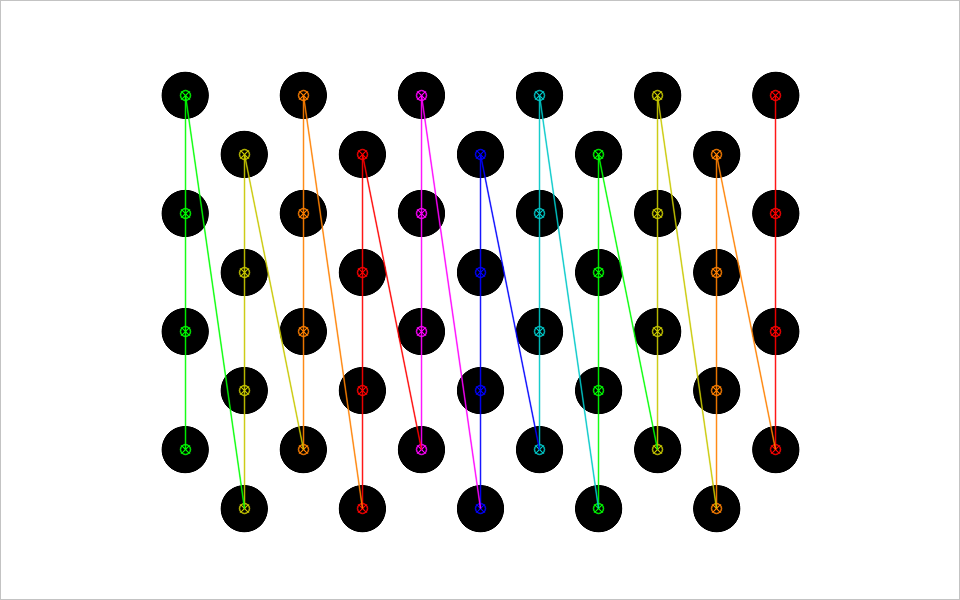
\includegraphics[height=3.25cm]{images/circles.png} }}
    \qquad
    \subfloat[\centering Projector calibration image (one for each target location), in image plane of camera (detections overlain).]{{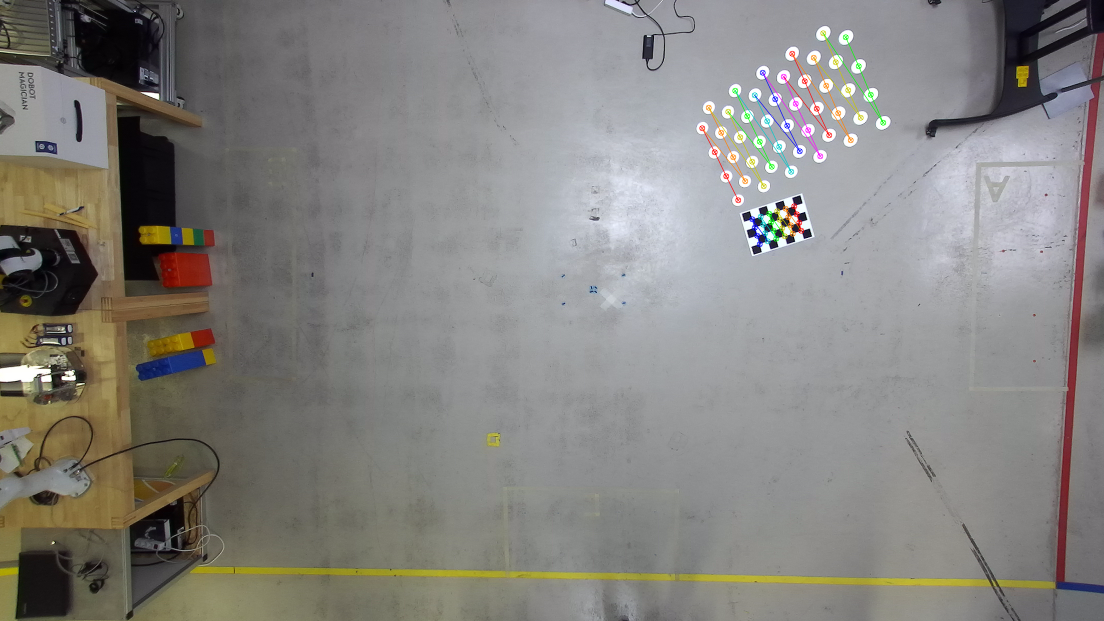
\includegraphics[height=3.25cm]{images/detections.png}}}
    \caption{Recovering 2D positions in support of projector calibration. (a) 2D positions of the 2D-3D correspondences to be used for calibrating the projector are obtained by detecting---in the image plane of the projector---the circle centers in the circles pattern image, projected by the projector to each of the target locations in the scene plane. (b) For each such target location, an image is acquired from the viewpoint of the camera and the circle centers of the projected circles pattern are detected, in the image plane of the camera. A chessboard pattern to be used for recovering the local scene plane is placed near the projected pattern, whose corners are likewise detected. Detected 2D projected circles pattern center points and chessboard corners overlain for illustration.} %At this stage, the chessboard is used to recover the local scene plane for each target location. Since the projected circles pattern lies in this plane, we are in a subsequent step able to rely on that plane to derive the 3D positions corresponding to the 2D projected circles pattern center points detected in the image.
    \label{fig:2d}
\end{figure}


\begin{figure}
    \centerline{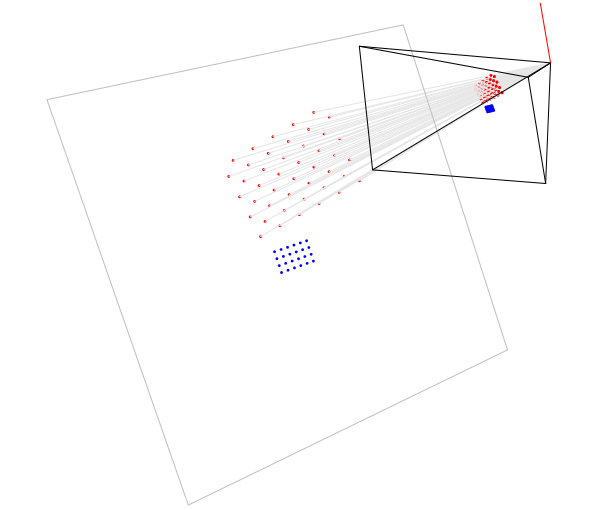
\includegraphics[scale=.35]{images/2d3d.png}}
    \caption{Scene plane (gray) recovered via spatial resection with respect to 2D-3D correspondences obtained using a chessboard pattern (blue); 3D circles pattern points obtained by intersection with the scene plane of back-projections (likewise gray) of circles pattern center points detected in the image plane (red). Note that the points in the figure are the points recovered for the projector calibration image in Figure~\ref{fig:2d}(b), acquired by the downwards-facing camera (frustum of the camera in black, with up vector in red).}
    \label{fig:3d}
\end{figure}


Calibration of a projector (or camera) in the sense we employ the term here\footnote{We are referring to a geometric calibration; not, e.g., to a color calibration.} renders one able to project a scene point~$\mathbf{X} \in \mathbb{R}^3$ to its corresponding pixel~$\mathbf{x} \in \mathbb{R}^2$ in the projector's (or camera's) image plane, or compute the `back-projection' of $\mathbf{x}$ (cf.\ Figure~\ref{fig:3d}), i.e., the ray from the projector's (or camera's) center of projection through $\mathbf{x}$ along which $\mathbf{X}$ must lie. Such a calibration can be expressed in terms of (i) a $3~\times{}~3$ calibration matrix~$\mathtt{K}$ derived from the projector's (or camera's) focal length and principal point \cite{Hartley2004}, and (ii) the coefficients of a lens distortion model used to correct for radial or tangential distortions caused by the lens system \cite{duane1971close}.

In practice, calibrating a camera relies on (i) establishing 2D-3D correspondences between pixels in the camera's image plane and corresponding points in the scene, and on (ii) using those correspondences as input to an optimization procedure that relies on bundle adjustment \cite{triggs1999bundle} to output the calibration matrix~$\mathtt{K}$, the associated lens distortion model coefficients, and, for each calibration image, the pose (i.e., position and orientation) of the camera relative to the 3D points \cite{Hartley2004,zhang2000flexible}. To calibrate a camera, a calibration surface such as a chessboard pattern is used to identify the correspondences. Calibration of a projector can be carried out in precisely the same manner insofar as step (ii) is concerned; the major difference in projector calibration relative to the calibrating a camera concerns the manner in which 2D-3D correspondences are identified, i.e., between pixels in the image plane of the projector and the corresponding points in the scene. A convenient consequence of the approach we take to identifying the 3D points of the 2D-3D correspondences needed for projector calibration is, for each target location, recovery of the pose (i.e., position and orientation) of (i) the projector and of (ii) the scene plane, both relative to the coordinate frame of the camera.

\paragraph{Camera calibration} The recovery of 2D-3D correspondences in support of camera calibration is carried out by relying on a planar calibration surface to automatically identify correspondences between the 3D points on the calibration surface and their 2D correspondences in the image plane. The classical calibration surface is a chessboard pattern. The 3D corner points of the chessboard are obtained \textit{a priori} in a coordinate system defined in the plane of the chessboard\footnote{E.g., $(0,0,0), (1.5,0,0), (3,0,0), \dots, (9,7.5,0)$ for a chessboard with $7~\times{}~6$ corners, with each square of length and width of 1.5 unit, respectively. Note that the units of the chessboard's 3D points give the units of the camera calibration, and---owing to how our projector calibration relies on the camera calibration---of the projector calibration as well.}, requiring knowledge only of the dimensions of the chessboard pattern and of the length of a side of a chessboard square. The corresponding 2D points are obtained, in the same order, using a specialized algorithm \cite{bradski2000opencv}. A set of calibration images is acquired, each with the calibration pattern visible in a different part of the image plane, and such that the center and all corners and edges of the image plane are covered, the camera's autofocus setting is off, and the camera's zoom factor remain fixed. 2D-3D correspondences are then recovered for each calibration image, and the resulting list is passed on as input to an optimization procedure that relies on bundle adjustment to yield the camera calibration matrix~$\mathtt{K}_\text{cam}$ and the associated lens distortion model coefficients. 

\paragraph{Projector calibration} As with camera calibration, projector calibration relies on 2D-3D correspondences, yet we obtain them in this case by projecting a pattern of circles. We rely on an algorithm to detect the circle pattern center points in the circles pattern image in the image plane of the projector \cite{bradski2000opencv}, giving the 2D positions of our 2D-3D correspondences (cf.\ Figure~\ref{fig:2d}(a)). We project the circles pattern image to each of the target locations, and use the camera to acquire a projector calibration image for each. Given a projector calibration image, we detect the circle centers of the \textit{projected} circles pattern (cf.\ Figure~\ref{fig:2d}(b)); given the scene plane (the recovery of which we shall return to in the paragraph that follows) and such a 2D circle center $\mathbf{x}$, its 3D correspondence is obtained by intersecting the back-projection of $\mathbf{x}$ with the scene plane (cf.\ Figure~\ref{fig:3d}). Since the algorithm that yields 2D circle centers does so in a consistent ordering, we thus obtain the 2D-3D correspondences between the projector's image plane and the scene required for projector calibration, yielding the projector calibration matrix~$\mathtt{K}_\text{proj}$.

We recover the scene plane via spatial resection by applying a PnP algorithm \cite{terzakis2020consistently} to the 2D-3D correspondences obtained using a chessboard pattern. Note that this step is separate from camera calibration, yet could well be carried out using the same calibration pattern used in the camera calibration step.\footnote{The critical point is that the pattern should ideally be coplanar with the local scene plane, meaning its height above the scene plane should not exceed a few millimeters.} While a single image of such a chessboard pattern placed on the floor could be sufficient if the floor is even, we place a chessboard pattern in close proximity to the projected circles pattern in each projector calibration image in order to recover the scene plane locally to each target location, in order to account for the possibility of an uneven floor.

The pose (i.e., position and orientation) of the projector, for each projector calibration image, is provided alongside $\mathtt{K}_\text{proj}$ by the aforementioned optimization procedure. Note that for a fixed projector with steerable mirror, given a projector calibration image, the recovered projector's pose is the pose the projector would have to have had to project to the given target location \textit{in the absence of the mirror}. As this is sufficient for our needs in Section~\ref{sec:approach:homography}, it is in this sense that our system is able to handle a projector equipped with a steerable mirror, without need for modeling the steerable mirror explicitly.

\subsection{Correcting for Projective Distortion}\label{sec:approach:homography}

If the projector is calibrated and its pose relative to the scene plane is known, a `virtual' projector (with the same calibration $\mathtt{K}$ and lens distortion coefficients) can be placed elsewhere relative to the scene plane. If we for a moment imagine that the projector---at its recovered pose---functions as a camera,\footnote{Recall that the calibration matrix~$\mathtt{K}$ enables computing both (i) the projection of a scene point to the image plane (the function of a camera), or (ii) the back-projection of a pixel in the image plane, giving a ray into the scene (along which a projector illuminates the scene with the given pixel).} then (i) projecting an image to the scene plane \textit{from the viewpoint of the virtual projector} and (ii) acquiring the resulting projected image from the viewpoint of the recovered projector gives the desired corrective warp. Projecting an image warped in this manner to the scene plane \textit{from the viewpoint of the recovered projector} then has the same effect as projecting the unwarped image to the scene plane from the viewpoint of the virtual projector. This warp can computed using a plane-induced homography, computed analytically as a function of the scene plane, the projector, and the virtual projector.

\begin{figure}
    \centering
    \subfloat[\centering Oblique view.]{{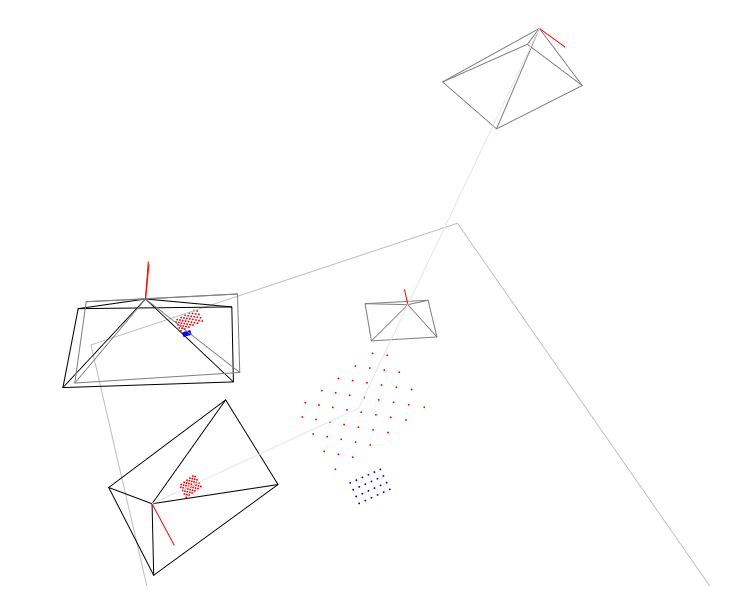
\includegraphics[height=4.2cm]{images/3.png}}}
    \qquad
    \subfloat[\centering Downwards view.]{{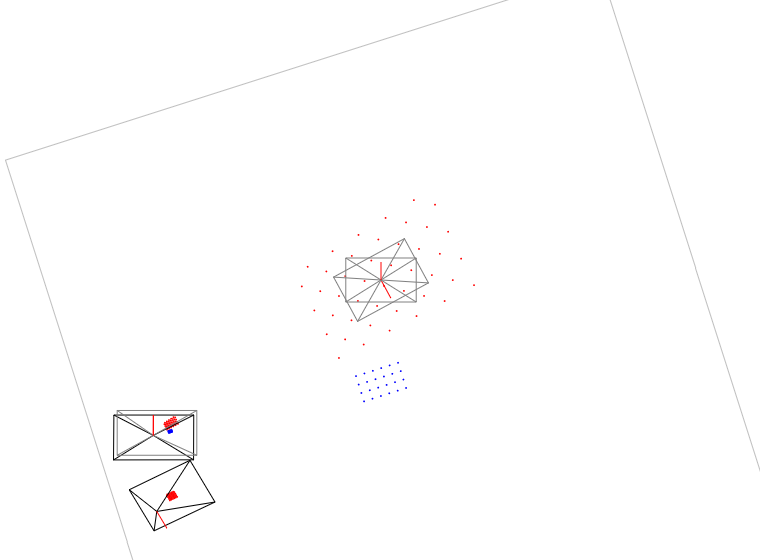
\includegraphics[height=4.2cm]{images/3_above3.png}}}
    \caption{The virtual camera is obtained by rotating the camera (top left, black) about its center of projection such that its optical axis be made parallel with the normal vector of the scene plane. The virtual projector is obtained by (i) rotating the projector (bottom left, black) about the point of intersection of its optical axis with the scene plane such that the optical axis be made parallel with the scene plane's normal vector, (ii) rotating the $X$- and $Y$-axes to align them with those of the virtual camera, and (iii) optionally translating along the normal direction to achieve the desired projected image dimensions.} %The virtual projector is thus rendered fronto-parallel with the ground plane and axially aligned with the virtual camera.
    \label{fig:virtualproj}
\end{figure}


\paragraph{Virtual projector} The placement of the virtual projector determines from which pose the image to be projected is to \textit{appear} to have been projected. This placement is produced according to a small handful of steps. First, we (i) rotate the camera about its center of projection to align its optical axis with the normal vector of the scene plane, giving a virtual camera likewise facing directly\footnote{A physical camera placed to face downwards is likely to not face downwards precisely; in contrast, the virtual camera's optical axis is aligned exactly with the scene plane's normal vector, rendering it fronto-parallel with respect to the scene plane.} downwards to the scene plane (cf.\ Figure~\ref{fig:virtualproj}). Next, we (ii) intersect the scene plane with the optical axis (i.e., the ray from the projector's center of projection through the center of the image plane); then, we (iii) rotate the projector's placement about that point of intersection, aligning the optical axis with the scene plane's normal vector and giving an initial virtual projector. Finally, we (iv) align the $X$- and $Y$-axes of the initial virtual projector with those of the virtual camera, which gives the virtual projector (cf.\ again Figure~\ref{fig:virtualproj}). The virtual projector is thus rendered fronto-parallel with the scene plane, enabling projection to the scene plane absent of projective distortions. Optionally, we additionally adjust the height above the scene plane of the virtual projector, in order to satisfy desired projected image dimensions provided in metric units.

Owing to the manner in which we place the virtual projector, the virtual projector's axes and thus the augmentation are aligned with the axes of the downward-facing camera; the placement of the camera thereby intuitively determines the principal axes according to which augmentations are placed. Note further that a consequence of placing the virtual projector by rotating about the point of intersection of the projector's optical axis with the scene plane is that the center of the projector's image plane remains invariant to the placement of the virtual projector, i.e., a steerable mirror can be aimed with respect to a point projected from the center of the projector's image plane, further facilitating placement.

\paragraph{Plane-induced homography} Let $\mathtt{K}_\text{proj}$ express the calibration matrix of the recovered projector and $(\mathtt{R}, \mathbf{t}) \in SE(3)$ the rigid body transformation that transforms points from the coordinate frame of the recovered projector to that of the virtual projector, for a given target location. Moreover, let $(\mathbf{n}^\top, -d)^\top$ give the scene plane, expressed in the coordinate frame of the recovered projector, where $\mathbf{n} \in \mathbb{R}^3$ is the scene plane's normal vector and $d = \mathbf{n}^\top\mathbf{X}$ for any point~$\mathbf{X}$ in the plane, so that $(\mathbf{n}^\top, -d) (\mathbf{X}^\top, 1)^\top = 0$. The transformation that distorts the image to be projected to the scene plane by the recovered projector such that it appear as if were projected to the scene plane by the virtual projector is given the by the $3~\times~3$ matrix
\begin{equation}
\mathtt{H} = \mathtt{K}_\text{proj}\left(\mathtt{R} - \frac{\mathbf{t}\mathbf{n}^\top}{d}\right)\mathtt{K}_\text{proj}^{-1},
\label{homgen}
\end{equation}
a form of `plane-induced' homography \cite{Hartley2004}. For convenience, we enable optional rotation of the image to be projected \textit{before} applying the homography, about the image center; that rotation, parameterized in degrees, is thus in effect likewise carried out intuitively relative to the placement of the camera.

\section{Evaluation}

We evaluate our approach by augmenting 15 locations across the floorspace at the Pilotfabrik\footnote{\url{https://www.pilotfabrik.at/}} of TU Vienna, a collaborative space for research on Industry 4.0 topics situated in Vienna, Austria. We contrast our approach with two variants of a baseline approach involving manual keystone correction (`Baseline A' and `Baseline B'), by aiming to place an image for each location aligned with the principal axes of the floorspace, absent projective distortions, and with the same dimensions (50~cm~$\times$~31.25~cm). Using our approach to carry out keystone correction analytically, we carried out all steps within a time budget of 15 min. Accordingly, we set 15 min to be the time budget of the first variant of the baseline approach (`Baseline A'), in which we carry out a \texit{manual} keystone correction using the software bundled with the steerable mirror system mounted alongside our projector. The second variant of the baseline approach (`Baseline B') is to again use the bundled software to carry out keystone correction manually, but to record how much time is necessary to produce augmentations within a mean tolerance of XX. All experiments were carried out jointly by the same experienced technician and assistant.

The hardware setup employed in the evaluation comprised a Panasonic PT-RZ660BE projector with a steerable mirror system---used to point the projection to each of the 15 locations---manufactured by Dynamic Projection Institute \cite{rupprecht2020information}. The steerable mirror system was bundled with the MDC-X software for steering the mirror, loading imagery, and optionally carrying out manual keystone correction, such that each position and (warped) image can be registered as a preset. In addition, we used a downward-facing Zed 2 stereo camera manufactured by Stereolabs, yet relied only on the left view. The floorspace used for our experiments measured dimensions of ca.\ 9~m~$\times$~4~m; the projector was mounted at approximately the center of this space, at a height of ca.\ 3.5 m.

\paragraph{Our approach} We began by carrying out a one-time\footnote{Note that once the camera is calibrated, that calibration can be reused if the camera's intrinsics remain fixed, i.e., no change is made to the zoom factor.} calibration of the camera, acquiring 10 camera calibration images (cf.\ Section~\ref{sec:approach:geometry}) and feeding the images as input to our camera calibration module. Separately, for each of the 15 target locations, we produced a projector calibration image (cf.\ again Section~\ref{sec:approach:geometry}) by projecting the circles pattern image to the location in question using the steerable mirror, placing a checkerboard pattern beside the projected pattern, and acquire the image using the downward-facing camera. We then fed these images alongside the output of the camera calibration module to our projector calibration module. For each of the target locations, the steerable mirror was made to point to that location, the circles pattern image was projected to the scene plane, an image was using the camera, and the location was registered in the MDC-X software as a preset. The output of the projector calibration module is a homography per input projector calibration image (cf.\ Section~\ref{sec:approach:homography}). Next, we warped the images to be projected to the respective locations using their corresponding homography, using a third dedicated custom module. These warped images were finally imported into the MDC-X software and associated with their respective location presets.

The total amount of time to carry out all the above steps amounted to ca.\ 15 min, with ca.\ 2 min going to acquisition of the camera calibration images, and ca.\ 5 min going to that of projector calibration images. The remainder of the time was spent running our modules or working with the MDC-X software.

\paragraph{Baseline A} ...

\paragraph{Baseline B} ...

\section{Conclusion}

We presented a spatial AR system for planar scenes that produces the effect of keystone correction analytically, and that intuitively places the desired augmentations in a manner aligned with the axes of an image of the scene acquired by a camera. Moreover, we showed our system to be able to handle a projector equipped with a steerable mirror, enabling wide-area factory floor augmentation exceeding the bounds of the projector's own immediate field of view. Our evaluation demonstrated ...

A natural extension of this work would be to address non-planar scenes. To handle non-planar scenes would call for a change in how scene geometry is recovered and how distortion of the image to be projected is carried out; projector calibration could, however, be left unchanged.

\bibliography{mybibfile}

\end{document}
